%% 
%% Copyright 2007-2020 Elsevier Ltd
%% 
%% This file is part of the 'Elsarticle Bundle'.
%% ---------------------------------------------
%% 
%% It may be distributed under the conditions of the LaTeX Project Public
%% License, either version 1.2 of this license or (at your option) any
%% later version.  The latest version of this license is in
%%    http://www.latex-project.org/lppl.txt
%% and version 1.2 or later is part of all distributions of LaTeX
%% version 1999/12/01 or later.
%% 
%% The list of all files belonging to the 'Elsarticle Bundle' is
%% given in the file `manifest.txt'.
%% 
%% Template article for Elsevier's document class `elsarticle'
%% with harvard style bibliographic references
\documentclass[12pt ,a4paper]{article}
%%%%%%%%%%%%%%%%%%%%%%%%%%%%%%%%%%%%%%%%%%%%%%%%%%%%%%%%%%%%%%%%%%%%%%%%%%%%%%%%%%%%%%%%%%%%%%%%%%%%%%%%%%%%%%%%%%%%%%%%%%%%

%% Use the option review to obtain double line spacing
%% \documentclass[authoryear,preprint,review,12pt]{elsarticle}

%% Use the options 1p,twocolumn; 3p; 3p,twocolumn; 5p; or 5p,twocolumn
%% for a journal layout:
%% \documentclass[final,1p,times,authoryear]{elsarticle}
% \documentclass[final,1p,times,twocolumn,authoryear]{elsarticle}
%% \documentclass[final,3p,times,authoryear]{elsarticle}
% \documentclass[final,3p,times,twocolumn,authoryear]{elsarticle}
%% \documentclass[final,5p,times,authoryear]{elsarticle}
%% \documentclass[final,5p,times,twocolumn,authoryear]{elsarticle}

\usepackage{amsmath}
\usepackage{amsfonts}
\usepackage{amssymb}
\usepackage[utf8]{inputenc}
\usepackage{url,hyperref,lineno,microtype,subcaption}
\usepackage{color,tensor,multirow,siunitx}
\usepackage[onehalfspacing]{setspace}
\usepackage{makecell}
\usepackage{graphicx}
\renewcommand{\cellalign}{cl}
% \usepackage{times}
\usepackage{caption}
\usepackage{lipsum}
\captionsetup[figure]{name=Fig., labelfont=bf}
\captionsetup[table]{name=Table, labelfont=bf}

\renewcommand{\cellalign}{cl}

\newcommand{\ds}{\displaystyle}
\newcommand{\nl}{\ \\ }
\newcommand{\ud}{\textrm{ d}}
\newcommand{\bs}{\bigskip}

\newcommand{\bu}{\mathbf{u}}
\newcommand{\bv}{\mathbf{v}}
\newcommand{\bx}{\mathbf{x}}
\newcommand{\be}{\mathbf{e}}
\newcommand{\bb}{\mathbf{b}}
\newcommand{\bk}{\mathbf{k}}
\newcommand{\bn}{\mathbf{n}}
\newcommand{\bR}{\mathbf{R}}

\definecolor{orange}{rgb}{1.0, 0.46, 0.09}
\definecolor{red}{rgb}{1,0,0}
\definecolor{blue}{rgb}{0,0,0.8}
\definecolor{green}{rgb}{0,0.5,0}
\newcommand{\emphc}[1]{\emph{\textcolor{red}{#1}}}
\newcommand{\hycom}{\textsc{hycom} }
\newcommand{\ie}{{\it i.e.}\ }
\newcommand{\eg}{{\it e.g.}\ }
\newcommand{\UV}{\mathbf{U}}
\newcommand{\todo}[1]{\textcolor{red}{TO DO: #1}}
\newcommand{\comment}[1]{\textcolor{orange}{#1}}
\usepackage[authoryear,round]{natbib}
%\newcommand{\modif}[1]{\textcolor{blue}{#1}}
% \renewcommand{\familydefault}{\sfdefault}
\usepackage{times}

\begin{document}
\section{Coral reefs}

\section{Coral reefs of Florida}

The Florida Reef Tract (FRT) spans over 580 km from the Dry Tortugas west of the Florida Keys to the St. Lucie Inlet in Martin County, constituting the third largest barrier reef in the world \citep{finkl2008shelf}. These reefs have a fauna and species richness typical of Caribbean reefs, including more than 40 species of stony corals \citep{banks2008reef,jackson2014status}. The northern half-section of the FRT consists of relic, Holocene framework reefs and indurated sand ridges harboring a rich but non-framebuilding fauna. Reefs in this area are separated into three shore-parallel reefs (inner, middle, outer) separated by sandy plains. Benthic cover is generally denser on the middle and outer reefs while the inner reef harbors some large patches of dense \textit{Acropora cervicornis}. The bouldering \textit{Montastraea cavernosa} is the dominant reef builder, but living hard coral cover is pretty low (below 6\%) \citep{banks2008reef}. The southern half-section is composed of chain of limestone islands (the Keys), sandbars and ancient coral reefs, where active carbonate deposition is taking place \citep{hoffmeister1968geology}.

Florida's Coral Reef (FCR) is of considerable importance to the economy of the state. \cite{johns2003socio} estimated the contribution of recreational users of natural and artificial reefs over the period June 2000 to May 2001 to have been US\$2.3 billion in sales and US\$1.1 billion in income. Moreover, recreational use of the reefs was evaluated to bring 36,500 full and part-time jobs. Focusing on natural reefs only, \cite{brander2013total} estimated the total coral reef values Florida to be US\$174 millions. However, this value might be underestimated as non-use value and indirect use values, such as support for coastal fisheries and coastal protection were not taken into account.

However, FCR has been heavily impacted by human activities including densely populated coastlines, high visitor numbers, polluted terrestrial run-off and overfishing \citep{jackson2014status}. Florida’s coral reefs have therefore declined significantly over the past decades due to anthropogenic impacts and numerous disease outbreaks \citep{jackson2014status}.

The Caribbean is considered as a disease "hotspot" because of the fast emergence, high prevalence, wide geographic distribution, and virulence of coral reef diseases in this area \citep{harvell2007coral}. Although they only represent 8\% of the total global coral reef area \citep{spalding1997new}, over 70\% of all disease and syndrome reports originate from the Caribbean.

Florida is a prime landfall target for tropical cyclones from June through November. Hurricanes that forms in June and July are usually weak while hurricanes occurring in August and September tend to become severe storms \citep{banks2008reef}. This is illustrated by Hurricane Irma, one of the strongest and costliest hurricanes on record in the Atlantic, that made landfall in Florida in September 2017 as a category 4 hurricane \citep{irmaNOAA, xian2018brief}. basin Hurricanes can influence the biota of coral reefs in many ways. The most obvious is wholesale destruction but hurricanes can also positively impact corals by facilitating the asexual recruitment of some species. However, some possible. Furthermore, hurricane-generated wave and currents have been hypothesized to transport silt and clay shoreward from deeper areas, causing burial of nearshore reefs on the continental shelf \citep{miller2008effects}

\begin{figure}
    \centering
    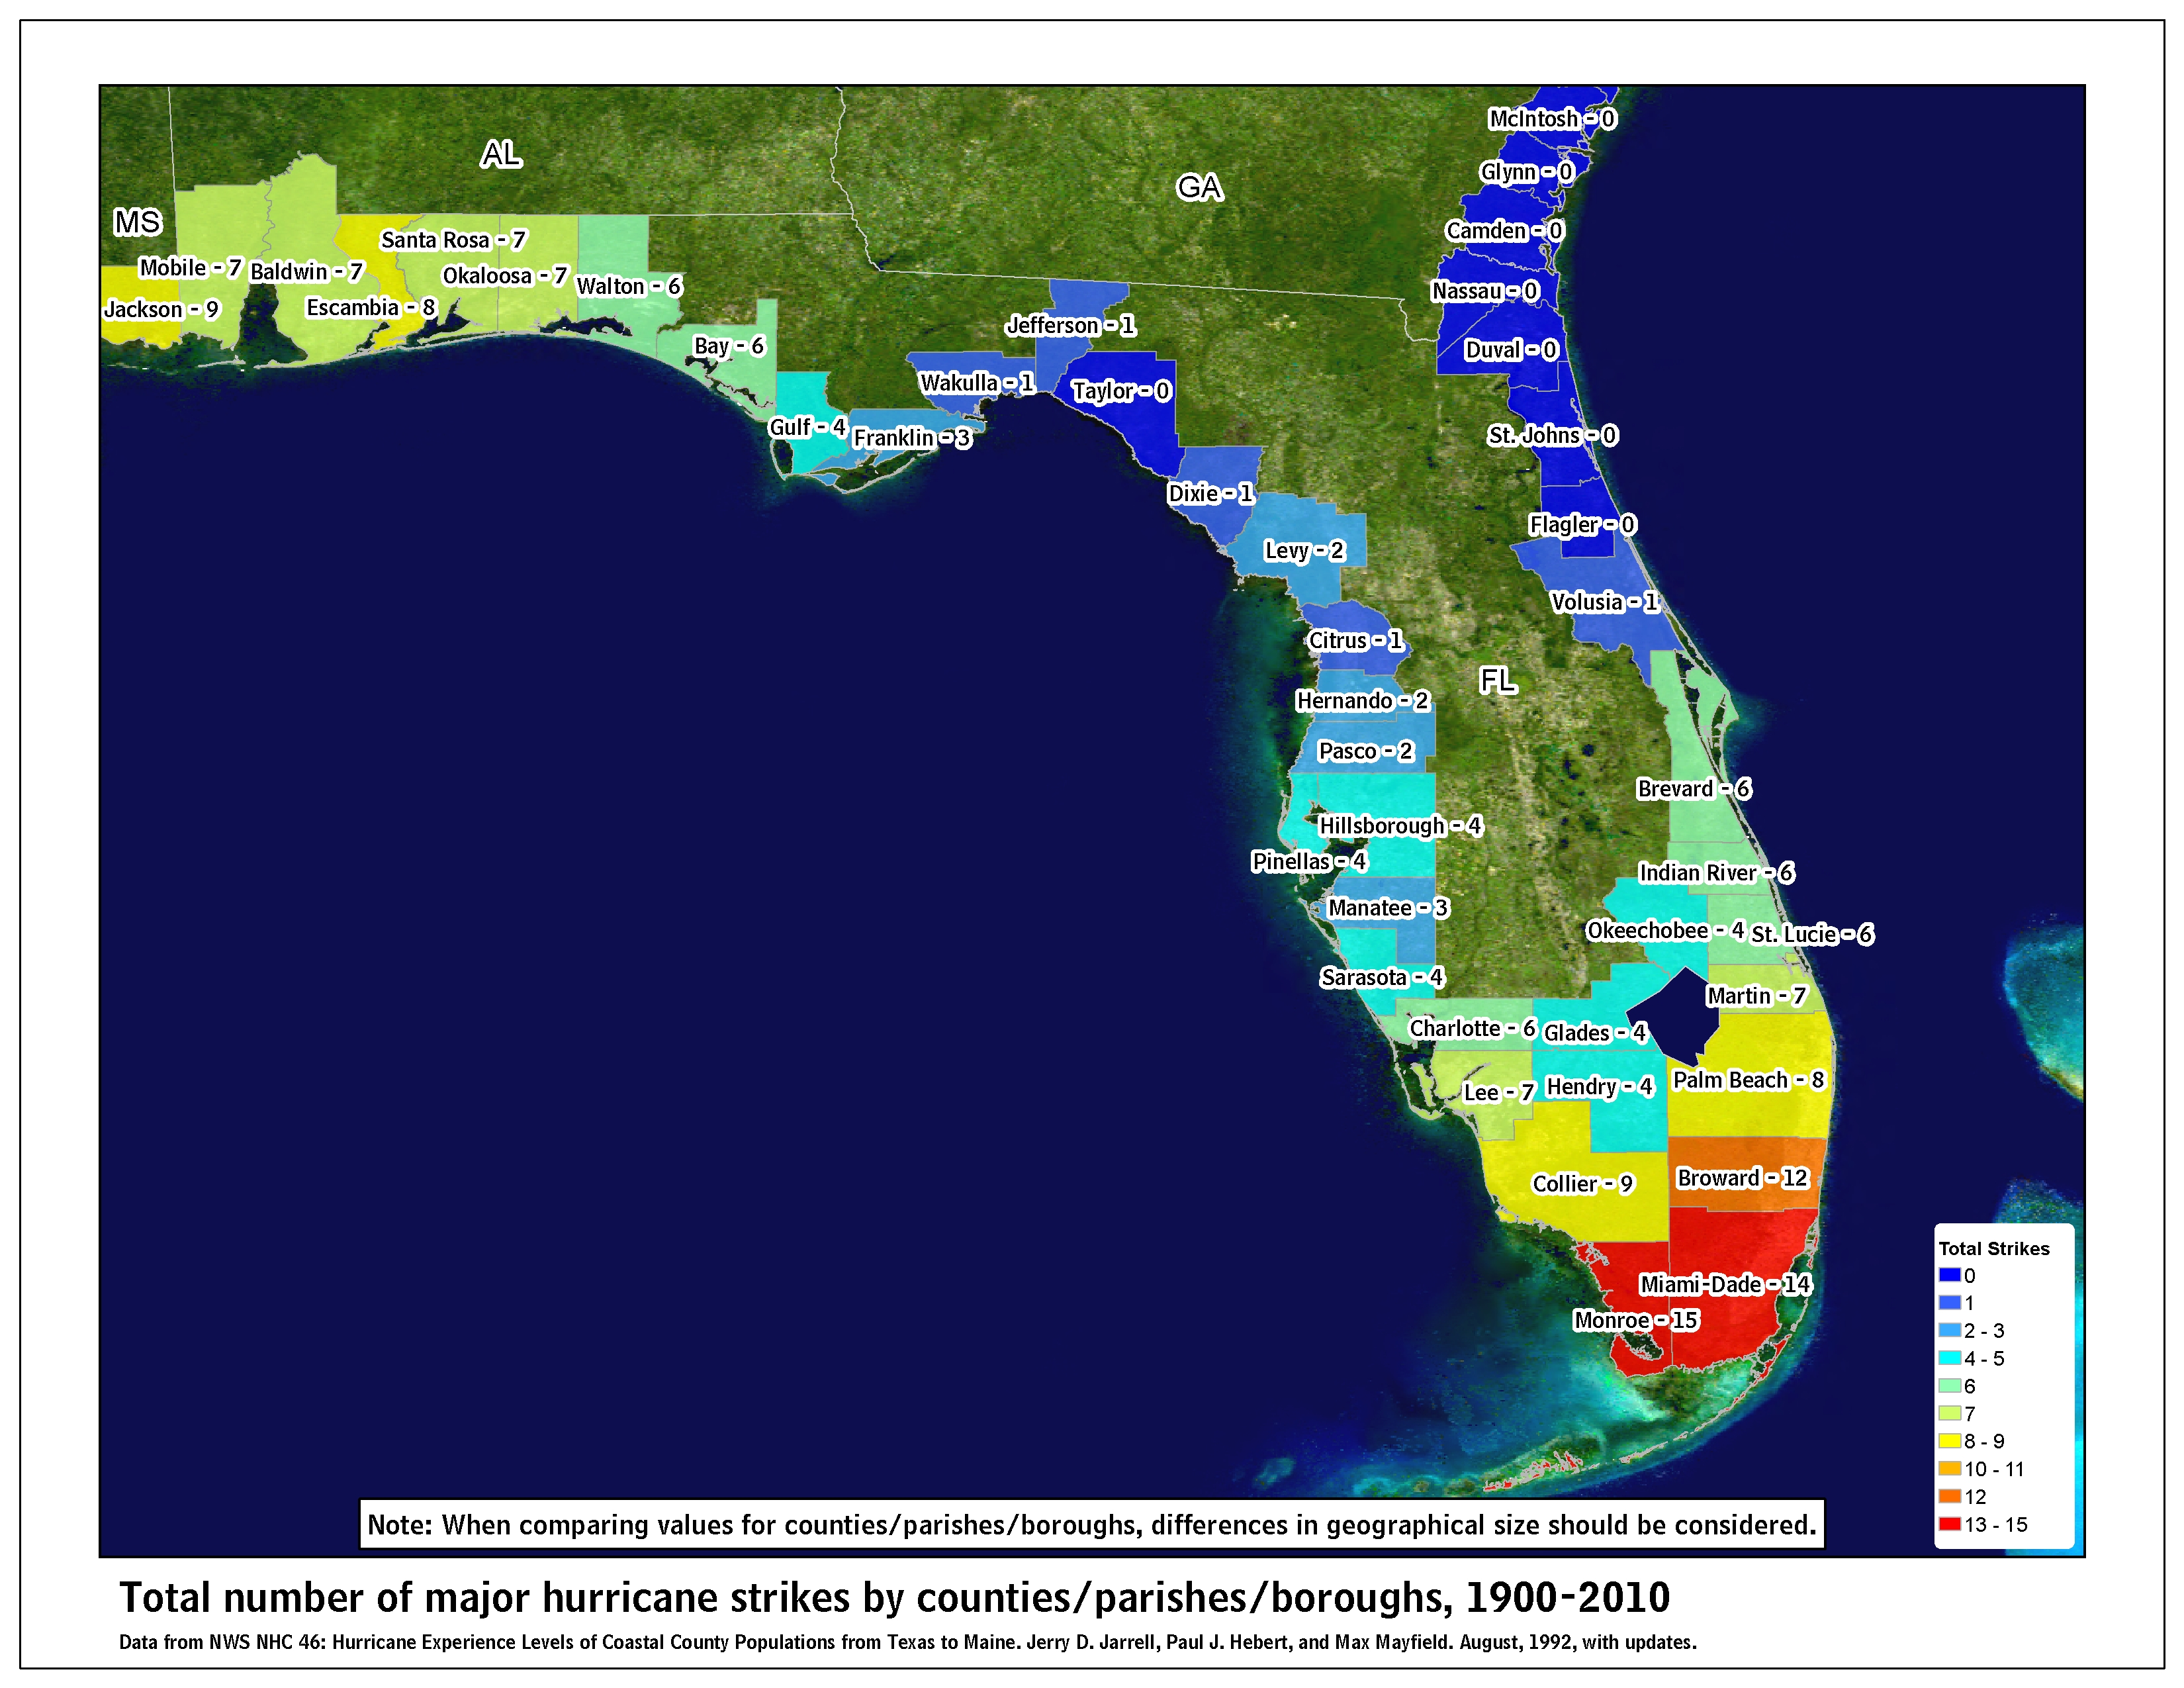
\includegraphics[width=\textwidth]{figures/hurricane_strikes.jpg}
    \caption{}
    \label{inro:landfall}
\end{figure}



\bibliographystyle{apalike} 
\bibliography{./biblio.bib}

\end{document}